\documentclass[11pt]{article}

\usepackage{booktabs}
\usepackage{float}
\usepackage{graphicx}
\usepackage{hyperref}

\begin{document}

\title{MNIST Exploration}
\author{Hang Wu}
\maketitle

\section{Classifier on original data}

\subsection{Configurations}
In this section, the neural network we are using has the following architecture:
\begin{verbatim}
    Conv2d([1,10,5*5]) -> MaxPooling -> ReLu ->
    Conv2d w. Dropout ([10, 20, 5*5) -> MaxPooling -> ReLu ->
    FullyConnected([320, 50])  -> BatchNormalization -> 
    FullyConnected([50, 10])
\end{verbatim}

We use Stochastic Gradient Descent (SGD) to optimize  the network parameters, with learning rate = 0.01, momentum = 0.5, and zero weight decay. The batch size is set to 100 and we train the network with 1 epoch. The model is implemented in the recently released PyTorch and results are obtained by averaging 5 rounds.

\subsection{Classification Result \& Discussions}
\paragraph{What is your test set error rate?} -

On the test set, the average negative log likelihood is 0.082 and the average classification error rate ( the percentage of wrongly classified samples) is 0.021.

\paragraph{What is the test set error rate for each class? Are some classes more challenging than others to distinguish from each other? Why?} -

The confusion matrix for the classification is shown in Tab. \ref{my-label} ($C[i,j]$ indicates the number of samples from class i that are classified as class j):

\begin{table}[ht]
\centering
\caption{Confusion Matrix}
\label{my-label}
\begin{tabular}{@{}lllllllllll@{}}
\toprule
  $\rightarrow$ & 0              & 1              & 2              & 3              & 4              & 5              & 6              & 7              & 8              & 9              \\ \midrule
0 & \textbf{0.992} & 0.001          & 0.002          & 0.000          & 0.000          & 0.000          & 0.002          & 0.001          & 0.002          & 0.000          \\
1 & 0.000          & \textbf{0.992} & 0.003          & 0.004          & 0.000          & 0.000          & 0.001          & 0.000          & 0.000          & 0.000          \\
2 & 0.001          & 0.002          & \textbf{0.984} & 0.004          & 0.002          & 0.001          & 0.001          & 0.004          & 0.002          & 0.000          \\
3 & 0.001          & 0.000          & 0.002          & \textbf{0.984} & 0.000          & 0.004          & 0.000          & 0.006          & 0.002          & 0.001          \\
4 & 0.000          & 0.001          & 0.001          & 0.000          & \textbf{0.978} & 0.000          & 0.003          & 0.000          & 0.001          & 0.016          \\
5 & 0.002          & 0.000          & 0.000          & 0.013          & 0.000          & \textbf{0.979} & 0.004          & 0.001          & 0.000          & 0.000          \\
6 & 0.008          & 0.003          & 0.001          & 0.000          & 0.001          & 0.006          & \textbf{0.978} & 0.000          & 0.002          & 0.000          \\
7 & 0.000          & 0.003          & 0.014          & 0.004          & 0.000          & 0.000          & 0.000          & \textbf{0.968} & 0.002          & 0.010          \\
8 & 0.003          & 0.001          & 0.003          & 0.002          & 0.001          & 0.009          & 0.001          & 0.004          & \textbf{0.970} & 0.005          \\
9 & 0.005          & 0.001          & 0.002          & 0.002          & 0.004          & 0.007          & 0.000          & 0.007          & 0.004          & \textbf{0.968} \\ \bottomrule
\end{tabular}
\end{table}

From the confusion matrix, we conclude that 7 and 9 are the most difficult classes, as 7 is easily confused with 2 and 9, and 9 is with 0,5,7, and 8. For a better treatment, we can analyze the cross entropy loss of predicting each class, as they represent the probability of each sample classified to 10 classes.

\paragraph{Based only on information gathered in the first epoch of training, do you think that the model would benefit from more training time? Why?} - 

As shown in Fig. \ref{fig:exp1}, the train losses are decreasing as more mini-batches are fed, however, it appears that the training hasn't converged to an almost flat line yet, so it could benefit from more training time.

\begin{figure}
    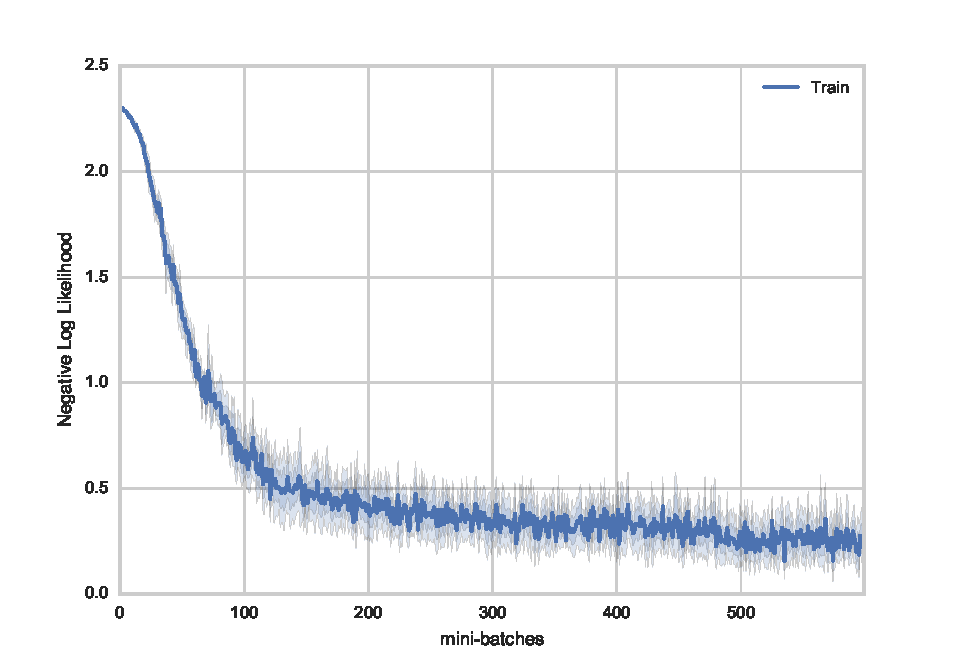
\includegraphics[width=.9\textwidth]{Figs/exp1}
    \caption{Train Losses in the first epoch}\label{fig:exp1}
\end{figure}

\paragraph{Besides training for a longer time, what would you do to improve accuracy?} -

Several methods can help improve accuracy, as suggested by literatures:

\begin{itemize}
    \item \textbf{Regularization} I originally tested a naive neural network without any regularization, and the classification error is averaged around 0.4, which is pretty poor. So I added dropout as a regularization \cite{srivastava2014dropout}. Other regularizations include: weight decay, early stopping \cite{goodfellow2016deep}.
    \item \textbf{Domain Specific Transformation} For natural images, some preprocessing may help improve the accuracy: random cropping, random perturbation of brightness, saturation, hue and contrast \cite{zhang2016understanding}. Data augmentation techniques including rotation, scaling, and flipping can also applied to training images.
    \item \textbf{Better Optimizers and Better Hyper-Parameters} AdaGrad \cite{duchi2011adaptive}, Adam \cite{kingma2014adam}, and AdaDelta \cite{zeiler2012adadelta} could help the network training converge faster. Tuning the learning rate can accelerate the convergence of the optimization process.
    %\item \textbf{Ensemble} Ensembles of deep networks are shown to improve performance \cite{goodfellow2016deep}.
    %\item \textbf{Pre-training} We can also adopt the greedy layer-wise pre-training to find a good initialization point \cite{bengio2007greedy}.
\end{itemize}

\section{Adding Image Noise}
\subsection{Configurations}
In this section, we tested several tricks in training deep networks, and vary the standard deviation of the noises added from 0 to 512. Fig. \ref{fig:exp2imgs} is a visual inspection of the effect of the noise. We can see that after the noise level reaches 512, the images are almost not identifiable, so we shall expect the classifiers output almost random outcomes.

\begin{figure}[ht]
    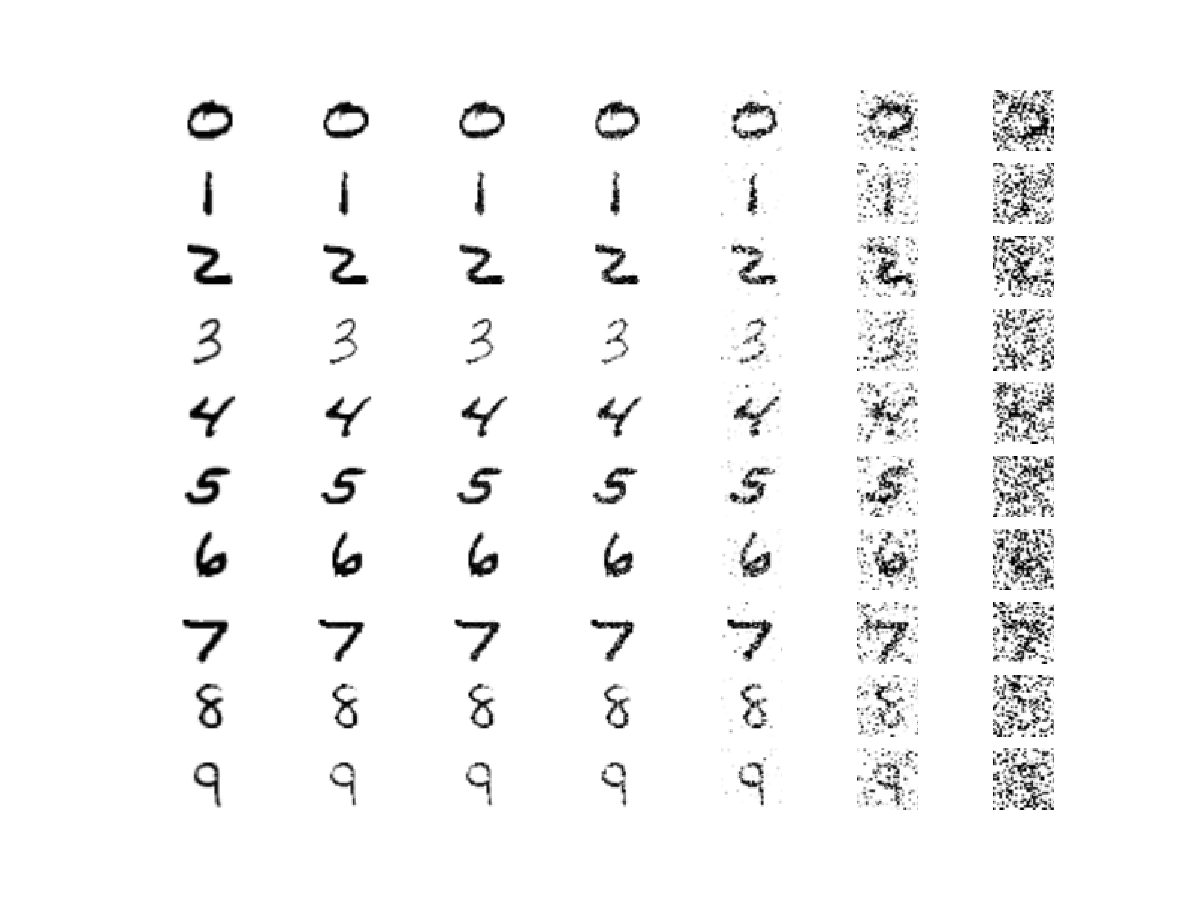
\includegraphics[width=.9\textwidth]{Figs/exp2_imgs}
    \caption{Adding noises with standard deviation from [0, 8, 32, 64, 128, 256, 512] to some sample images.}\label{fig:exp2imgs}
\end{figure}


Specifically, the network architectures include

\begin{itemize}
    \item Naive - Only convolution, ReLu, and fully-connected layers are used.
    \item BN - Adding batch normalization layer before the first fully-connected layer.
    \item DO - Adding dropout to the naive network.
    \item WD - Set the weight decay of SGD to 0.005 instead of 0\footnote{Parameter set as suggested by \url{http://caffe.berkeleyvision.org/gathered/examples/mnist.html}}.
    \item BN + DO - The network structure shown in the first section.
    \item BN + DO + WD - Combining all tricks.
\end{itemize}

All the results here are obtained by averaging 5 rounds, but to keep the figures clean, we only show here the version without error bars.

\subsection{Classification Result}
\begin{figure}
    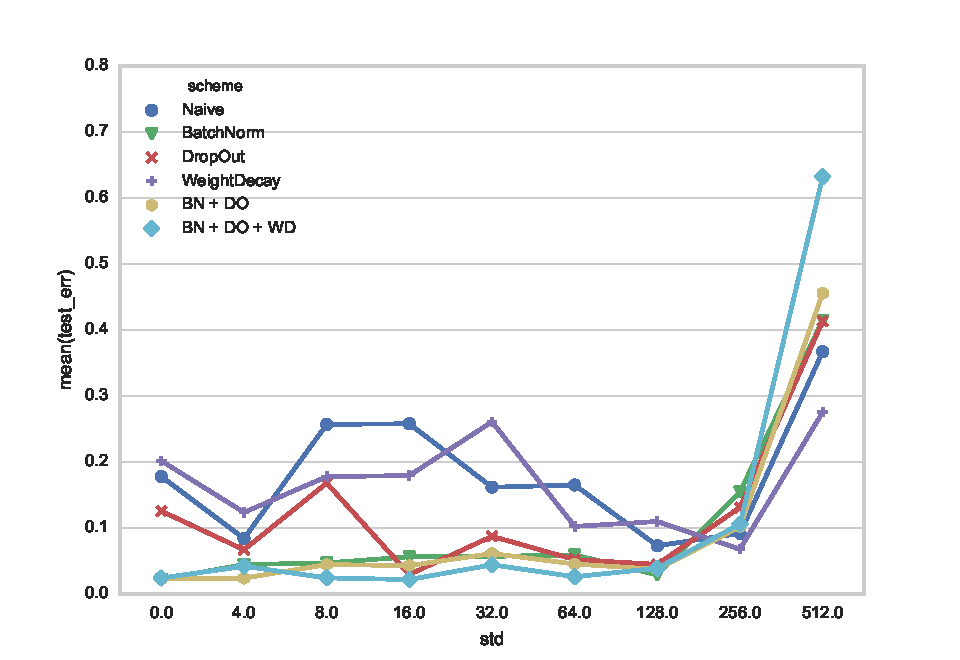
\includegraphics[width=.9\textwidth]{Figs/exp2_1}
    \caption{Classification Result with Image Noise}\label{fig:exp21}
\end{figure}
The figure \ref{fig:exp21} shows that the naive model and the weight-decay version is highly unstable, and dropout version performs slightly better. The rest three versions, which all include batch normalization, are much more robust to image noise. By comparing between these three versions, the benefit of introducing dropout, or weight decay, is not very significant.

All versions corrupt after the image noise reaches 512, two times of the maximum pixel values. 

\subsection{Discussions}
\paragraph{What are the implications of the dependence of accuracy on noise if you were to deploy a production classifier? How much noise do you think a production classifier could tolerate?} -

We need to decrease the magnitude and variance of the noise with preprocessing, and adding regularizations and batch normalization layers to prevent the network from overfitting. Obtaining more training data will also help reduce the effect of the noise. With batch normalization, I would say a standard deviation less than 100 seems okay.

\paragraph{Do you think that Gaussian noise is an appropriate model for real-world noise if the characters were acquired by standard digital photography? If so, in what situations? How would you compensate for it?} -

Gaussian noise may not be the most appropriate type. Several other types of noises are present in digital photography: besides Gaussian noises, there are salt-and-pepper (impulsive noises caused by analog-to-digital conversion), quantization noise (from continuous-to-discrete conversion), and shot noise (Poisson distribution noise). 

Besides batch normalization, applying filtering, for example, low-pass filtering and median filtering, could help reduce the noise as a preprocessing step \cite{kaur2015noise}. We can also train deep networks for each type of the noise, and output the ensemble of these networks as the prediction.

\paragraph{Is the accuracy of certain classes affected more by image noise than others? Why?} -
\begin{figure}[H]
    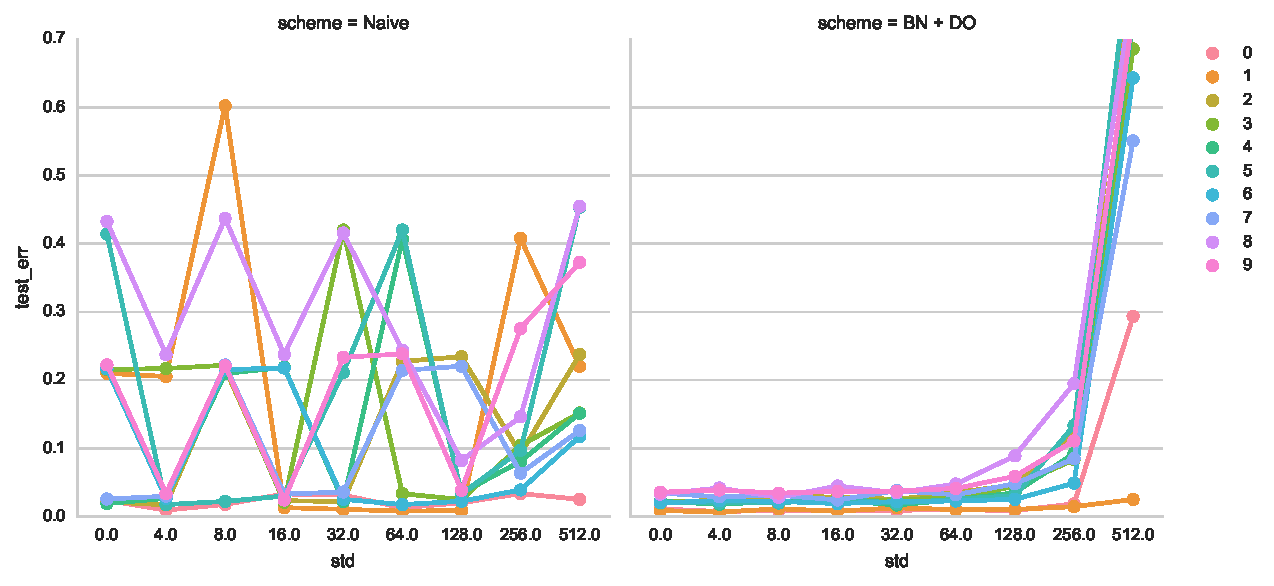
\includegraphics[width=.9\textwidth]{Figs/exp2_2}
    \caption{Classification Result with Image Noise}\label{fig:exp22}
\end{figure}
As shown in Fig. \ref{fig:exp22}, the naive model is performing unstable so we really cannot draw conclusions from it. With BN + DO, the performance is more consistent: in the long term, as the standard deviation goes up, the least robust classes are 8, while 1 is the most robust to the noise.

\section{Adding Label Noise}
\subsection{Configurations \& Results}
Xiao et el. \cite{xiao2015learning} suggests there are three settings w.r.t label noise $\tilde{y}$:
\begin{enumerate}
    \item The label is noise free
    \item The label $\tilde{y}$ takes an independent random value other than the original label $y$
    \item The label $\tilde{y}$ takes some confusing values, that are dependent upon the original label $y$
\end{enumerate}

In our experiments, we added the second type of noises, and the original labels are mapped to \{ 7, 9, 0, 4, 2, 1, 3, 5, 6, 8\} . All the other configurations are the same as in the first section.

\begin{figure}
    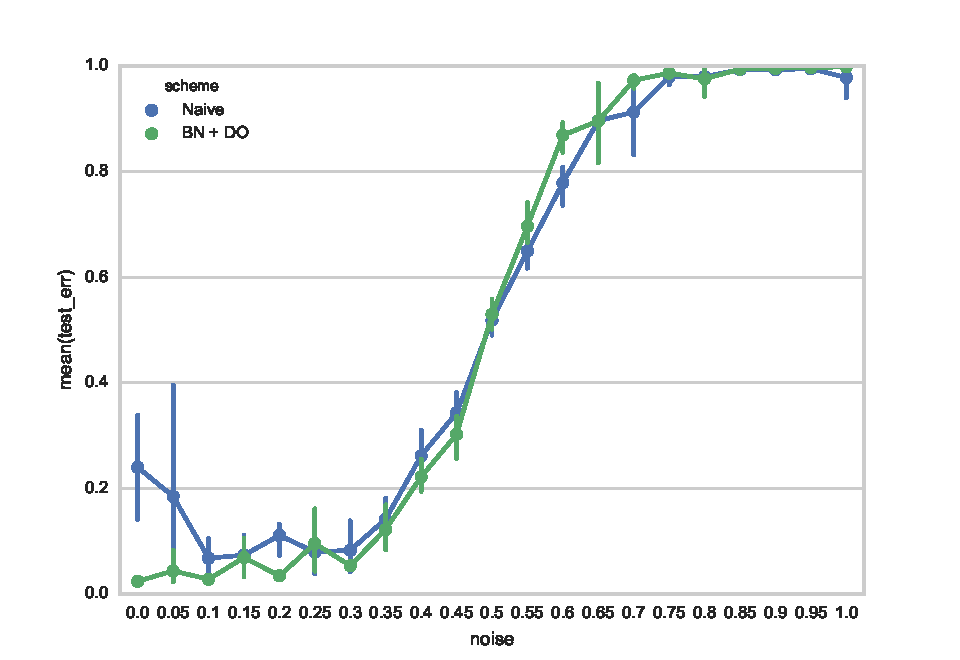
\includegraphics[width=.9\textwidth]{Figs/exp3}
    \caption{Classification Result with Label Noise}\label{fig:exp3}
\end{figure}

\paragraph{How important are accurate training labels to classifier accuracy?}
As shown by Fig. \ref{fig:exp3}, with smaller label noise ( $< 20\%$), the algorithm can perform quite robust, but as the label noises become larger than $20\%$, the errors are increasing fast, and will classify all samples wrong when the noises are greater than $80\%$.

\paragraph{How would you compensate for label noise? Assume you have a large budget available but you want to use it as efficiently as possible.} -

If we are able to re-label some of the images, we may adopt the active learning framework \cite{settles2010active}: each round, we ask our learning algorithm to actively query the user/ physicians for labels, for the images the algorithm are most unsure.

Otherwise, we need to make some assumptions on the noise generation process. Several literature deal with the label noises, and they assume a probabilistic model of the generation of label noise. We here discuss some recent ones:

1. Xiao et al. \cite{xiao2015learning} assumes that $p(\tilde{y} , y,z) = p(\tilde{y} | y,z) p(y|x) p(z|x)$, where $z$ denotes the three types of noise in the previous subsection, and $x$ is the feature of the image. With such assumption, the authors add another CNN to model the probability $p(z|x)$, and the $p(\tilde{y} | y,z)$ can be inferred via EM algorithm.

2. Reed et al. \cite{reed2014training} deals with the label permutation where $p(\tilde{y} = i | y =j) $ is a constant, and an additional loss of estimating such matrix is added to the network.

3. Goldberg et al. \cite{gold2017training} follows the assumption of \cite{reed2014training}, and directly estimating $p(\tilde{y} = i) = \sum p(\tilde{y} = i | y = j) p(y = j | x)$ via EM-like algorithm (the implementation is by adding a layer and performing back-propagation).

\paragraph{How would you quantify the amount of label noise if you had a noisy data set?} -

\begin{figure}[!ht]
    \centering
    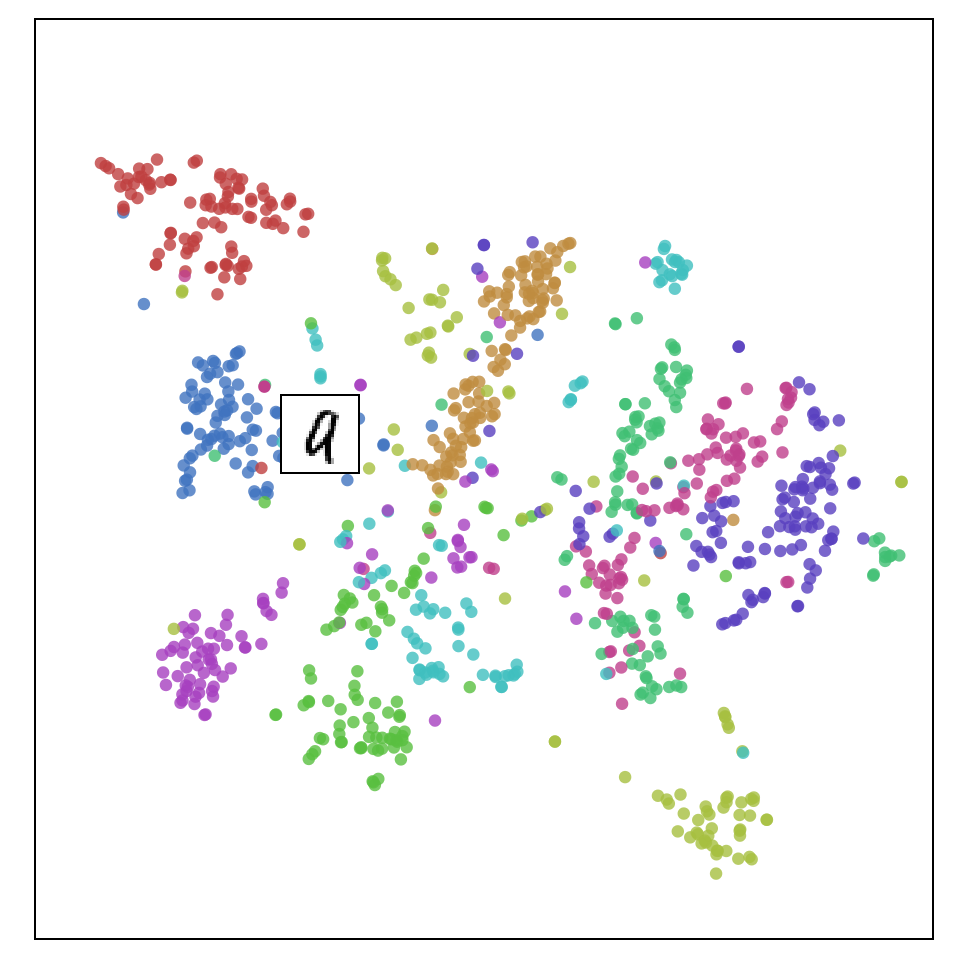
\includegraphics[width=.8\textwidth]{Figs/tsne}
    \caption{Visualization of MNIST data using t-SNE \cite{1_olah_2017}. The shown 9 is an outlier in the cluster of 4's.}
\end{figure}


If we follow the approach of active learning, the number of queries made can be a proxy for the noise in labels. For noise with special assumptions, we can estimate the probability $p(z|x)$, or the off-diagonal matrix entries to quantify the amount of noise.

We can also perform a clustering on all the images (followed by a low-dimension embedding for visualization) to inspect the coherence of each cluster, and understand the noise of labels. For example, Fig. is a visualization of t-SNE \cite{maaten2008visualizing} on MNIST dataset provided by \cite{1_olah_2017}. We can spot some of the outliers in each cluster to understand the label noise in our dataset.


\paragraph{If your real-world data had both image noise and label noise, which would you be more concerned about? Which is easier to compensate for?} -

I would be more concerned about label noise, as if the label noise are too prevalent, we cannot learn a meaningful classifier, while with image noise, we can adopt several simple preprocessing to reduce the influence of image noise.

\bibliographystyle{plain}
\bibliography{ref.bib}

\end{document}
